\documentclass[]{article}
\usepackage[T1]{fontenc}
\usepackage{lmodern}
\usepackage{amssymb,amsmath}
\usepackage{ifxetex,ifluatex}
\usepackage{fixltx2e} % provides \textsubscript
% use upquote if available, for straight quotes in verbatim environments
\IfFileExists{upquote.sty}{\usepackage{upquote}}{}
\ifnum 0\ifxetex 1\fi\ifluatex 1\fi=0 % if pdftex
  \usepackage[utf8]{inputenc}
\else % if luatex or xelatex
  \ifxetex
    \usepackage{mathspec}
    \usepackage{xltxtra,xunicode}
  \else
    \usepackage{fontspec}
  \fi
  \defaultfontfeatures{Mapping=tex-text,Scale=MatchLowercase}
  \newcommand{\euro}{€}
\fi
% use microtype if available
\IfFileExists{microtype.sty}{\usepackage{microtype}}{}
\usepackage{graphicx}
% Redefine \includegraphics so that, unless explicit options are
% given, the image width will not exceed the width of the page.
% Images get their normal width if they fit onto the page, but
% are scaled down if they would overflow the margins.
\makeatletter
\def\ScaleIfNeeded{%
  \ifdim\Gin@nat@width>\linewidth
    \linewidth
  \else
    \Gin@nat@width
  \fi
}
\makeatother
\let\Oldincludegraphics\includegraphics
{%
 \catcode`\@=11\relax%
 \gdef\includegraphics{\@ifnextchar[{\Oldincludegraphics}{\Oldincludegraphics[width=\ScaleIfNeeded]}}%
}%
\ifxetex
  \usepackage[setpagesize=false, % page size defined by xetex
              unicode=false, % unicode breaks when used with xetex
              xetex]{hyperref}
\else
  \usepackage[unicode=true]{hyperref}
\fi
\hypersetup{breaklinks=true,
            bookmarks=true,
            pdfauthor={},
            pdftitle={},
            colorlinks=true,
            citecolor=blue,
            urlcolor=blue,
            linkcolor=magenta,
            pdfborder={0 0 0}}
\urlstyle{same}  % don't use monospace font for urls
\setlength{\parindent}{0pt}
\setlength{\parskip}{6pt plus 2pt minus 1pt}
\setlength{\emergencystretch}{3em}  % prevent overfull lines
\setcounter{secnumdepth}{0}

\author{}
\date{}

\begin{document}

\section{Research Data Management
101}\label{research-data-management-101}

\subsection{Michelle Hudson \& Kristin
Bogdan}\label{michelle-hudson-kristin-bogdan}

\subsubsection{CSSSI workshop Feb 21
2014}\label{csssi-workshop-feb-21-2014}

\subparagraph{\url{https://github.com/michellehudson/datamanagement/}}\label{httpsgithub.commichellehudsondatamanagement}

\section{Description:}\label{description}

This two-hour workshop will provide an overview of the data lifecycle
and the critical steps within it that need to be addressed to ensure
integrity of research data. It is appropriate for students and faculty
in all disciplines, however, the constrained time-frame and high level
overview of the issues only warrant a few in-depth examples of tools and
resources for specific disciplines. The workshop will focus on general
good practices for data management that span disciplines. There will be
Q\&A time for specific questions, and attendees are always welcome to
follow up with instructors or other specialist for more tailored data
management instruction or assistance.

\begin{figure}[htbp]
\centering
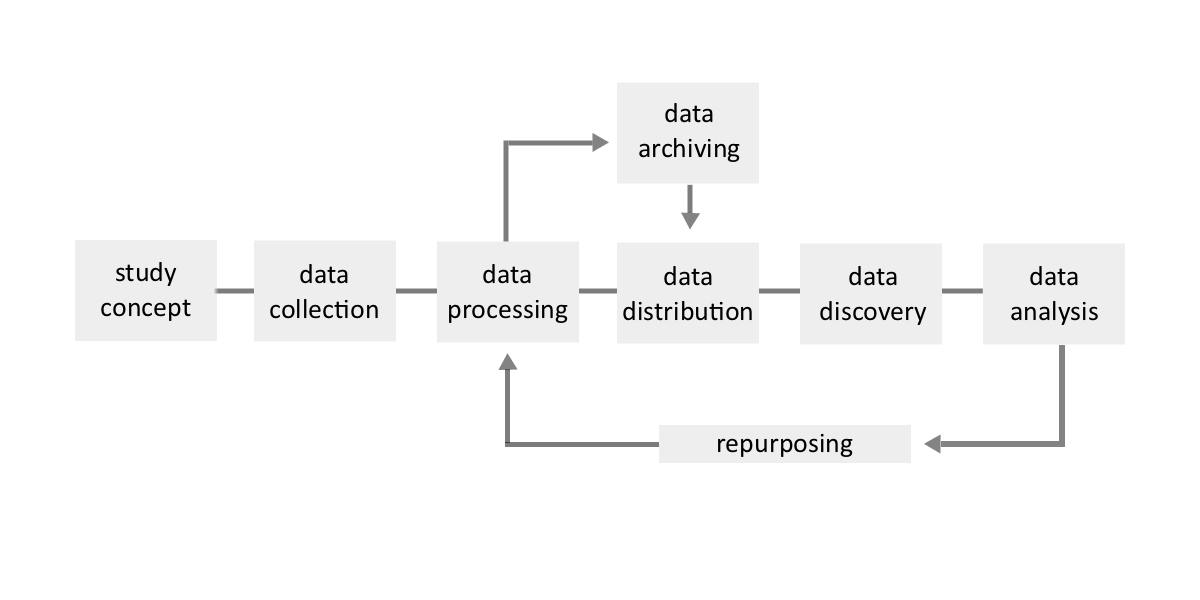
\includegraphics{ddilifecycle.png}
\caption{DDI lifecycle model}
\end{figure}

\section{General format:}\label{general-format}

Using the DDI data lifecycle model as a guide, we'll cover the following
questions:

\begin{enumerate}
\def\labelenumi{\arabic{enumi}.}
\itemsep1pt\parskip0pt\parsep0pt
\item
  What does this stage of the data lifecycle involve?
\item
  What resources are available for doing it well at Yale (\& elsewhere)?
\item
  What are guidelines for managing data at this stage?
\end{enumerate}

\section{Outline:}\label{outline}

\begin{enumerate}
\def\labelenumi{\arabic{enumi}.}
\itemsep1pt\parskip0pt\parsep0pt
\item
  What is data?
\item
  Why manage it?
\item
  Study concept
\item
  Data collection
\item
  Data processing
\item
  Data archiving
\item
  Data distribution
\item
  More resources
\item
  Q\&A
\end{enumerate}

\section{What is research data?}\label{what-is-research-data}

Research data is defined as ``the recorded factual material commonly
accepted in the scientific community as necessary to validate research
findings.'' OMB Circular A-110.

There are four types of research data:

\begin{enumerate}
\def\labelenumi{\arabic{enumi}.}
\itemsep1pt\parskip0pt\parsep0pt
\item
  Observational: captured in real time, usually irreplaceable (sensor
  readings, telescope images, sample data, surveys).
\item
  Experimental: data from lab equipment, can be reproducible but may be
  expensive (gene sequences).
\item
  Simulation: data generated from test models (climate models).
\item
  Derived or compiled: reproducible but expensive (data mining, compiled
  databases).
\end{enumerate}

Research data comes in many formats of information: documents,
spreadsheets, field notebooks, survey responses, audio and video
recordings, images, film, specimens, software code, and can be
structured and stored in a variety of file formats.

\section{Why manage research data?}\label{why-manage-research-data}

There are many reasons why good data management is important for your
research career, ranging from long-term effects on the future of science
to personal productivity and accomplishment.

\subsection{Transparency, integrity, and
reproducibility:}\label{transparency-integrity-and-reproducibility}

Managing data and making it accessible by peers decreases the chances of
an article being retracted because of falsified or missing data sets.
Reproducibility is a fundamental part of scientific research, and
failing to make all the components of a research study available makes
reproducibility impossible.

\subsection{Compliance:}\label{compliance}

Data management plans are required by funding agencies, and there is
increased expectation that the products of federal funding will be
required to be accessible to the public. In addition, many journals are
requiring data deposit before an article may be published.

\subsection{Personal \& professional
benefits:}\label{personal-professional-benefits}

If data is managed within your lab, research group, or simply
well-organized for your own use, you will save time, energy, and
resources. All members of the team will have an understanding of the
well-documented processing and analysis of the project's data, and be
able to carry out their research components more effectively. Sharing
research data is now regarded as an integral and valuable part of the
research process, and archiving your data in a repository will allow
other researchers to build upon your work and cite you in the process.

\section{Study concept}\label{study-concept}

\subsection{What does this stage
involve?}\label{what-does-this-stage-involve}

This is the planning process for a study. It involves formulating a
research question and deciding on the methods you want to use to execute
your study. It may include submitting a grant to get funding. Some
grants require data management plans to be submitted as part of the
proposal.

\subsection{What tools and resources are
available?}\label{what-tools-and-resources-are-available}

\paragraph{\href{https://dmp.cdlib.org/}{DMPTool}:}\label{dmptool}

Yale is a DMPTool partner. Logging in with your Yale ID and password
will give you access to the DMPTool, which will give you an overview of
funder requirements (for various NSF, NIH, and other directorates and
divisions), and walk you through building a data management plan, asking
the right questions along the way. In the next iteration of the tool,
we'll be able to further customize it with Yale-specific resources.

\paragraph{\href{http://csssi.yale.edu/dmp}{DMP Consultation
Group}:}\label{dmp-consultation-group}

If you have to submit a DMP as part of a grant proposal and have trouble
using the DMPTool or answering questions you think are critical to the
good management of data, you can contact the DMP Consultation Group for
help. This group can review written plans and offer feedback, or connect
you with more resources at Yale you might be able to cite or consider
including in your plan to make a stronger proposal.

\paragraph{\href{http://csssi.yale.edu/csssi-statistical-consultants-schedule}{StatLab
consultants}:}\label{statlab-consultants}

Even if you aren't submitting a grant proposal, it's a good idea to come
to the StatLab at the beginning of your project. If you know what
analyses you want to do on your data, the StatLab can make sure you set
out to collect your data correctly. If you anticipate using StatLab
services near the end of your project, it's much easier for them if you
connect in the beginning of the project, as well.

\section{Data collection \&
documentation}\label{data-collection-documentation}

\subsection{What does this stage
involve?}\label{what-does-this-stage-involve-1}

This stage involves all the collection and subsequent documentation of
your data, and may involve collaboration with other people. There aren't
a lot of collaborative online spaces for data collection, but we can
discuss a few, and some general guidelines for documenting your research
well.

\subsection{Study-level description}\label{study-level-description}

\begin{enumerate}
\def\labelenumi{\arabic{enumi}.}
\itemsep1pt\parskip0pt\parsep0pt
\item
  Context of the data collection (project history, aim, objectives, and
  hypotheses)
\item
  Data collection methods (sampling, data collection process,
  instruments used, hardware and software used to collect data, scale
  and resolution, temporal and geographic coverage, secondary data
  sources used, if any)
\item
  Data set structure -- of files, study cases, and relationships between
  files
\item
  Changes made to data over time
\item
  Information on access and use conditions or data confidentiality
\end{enumerate}

\subsection{File-level description}\label{file-level-description}

\begin{enumerate}
\def\labelenumi{\arabic{enumi}.}
\itemsep1pt\parskip0pt\parsep0pt
\item
  Names, labels, and descriptions for variables, records, and their
  values
\item
  Definition of codes \& classification schemes used
\item
  Codes of and reasons for missing values
\end{enumerate}

\subsection{What tools and resources are
available?}\label{what-tools-and-resources-are-available-1}

\subsubsection{Yale-supported:}\label{yale-supported}

\paragraph{\href{http://its.yale.edu/services/collaboration-and-file-sharing/box-yale}{Box}:}\label{box}

Box is a document-sharing cloud service available to everyone at Yale
and is supported by Yale ITS. See the link for questions about security
and size limits.

\paragraph{\href{http://its.yale.edu/services/research-technologies/elab-notebook/labarchives-faqs}{LabArchives}:}\label{labarchives}

LabArchives is an electronic lab notebook solution available to everyone
at Yale and is supported by Yale ITS.

\paragraph{\href{http://its.yale.edu/services/email-and-calendars/eliapps-google-apps-education}{EliApps}:}\label{eliapps}

EliApps may be an appropriate place to collaborate for simple
spreadsheets and forms for non-sensitive data.

\paragraph{\href{http://its.yale.edu/services/web-and-application-services/qualtrics-survey-tool}{Qualtrics}:}\label{qualtrics}

Qualtrics is robust survey building software, is available to everyone
at Yale, and is supported by Yale ITS.

\subsubsection{Additional services \&
software:}\label{additional-services-software}

\paragraph{\href{https://github.com/}{GitHub}:}\label{github}

GitHub is a free or paid service, popular for writing and sharing
software code, and can be used to track changes to files and work with
multiple collaborators. GitHub is not supported by Yale ITS.

\paragraph{\href{https://knb.ecoinformatics.org/morphoportal.jsp}{Morpho}:}\label{morpho}

Morpho was developed for data management in ecology.

\paragraph{\href{http://earthcube.org/}{Earthcube}:}\label{earthcube}

Earthcube is a community driven data and knowledge management system
that will allow for data sharing across the geosciences.

\paragraph{\href{http://www.colectica.com/}{Colectica}:}\label{colectica}

Colectica is software that helps design, document, and publish
statistical data and survey research using open data standards.

\subsection{Guidelines:}\label{guidelines}

\begin{enumerate}
\def\labelenumi{\arabic{enumi}.}
\itemsep1pt\parskip0pt\parsep0pt
\item
  Spreadsheets vs.~databases: see the upcoming workshop on database
  design: 4/18/2014, 1:30 - 3:30 CSSSI.
\item
  Consistency: whatever you do, stick with it.
\item
  Level of detail: decide how much detail you'll need now and in the
  future.
\end{enumerate}

\subsection{Example:}\label{example}

The codebook for the \href{http://www3.norc.org/GSS+Website/}{General
Social Survey} is an enormous document that helps researchers use the
data effectively and ensures that every variable is described.

\subsection{Reminder!}\label{reminder}

\begin{figure}[htbp]
\centering
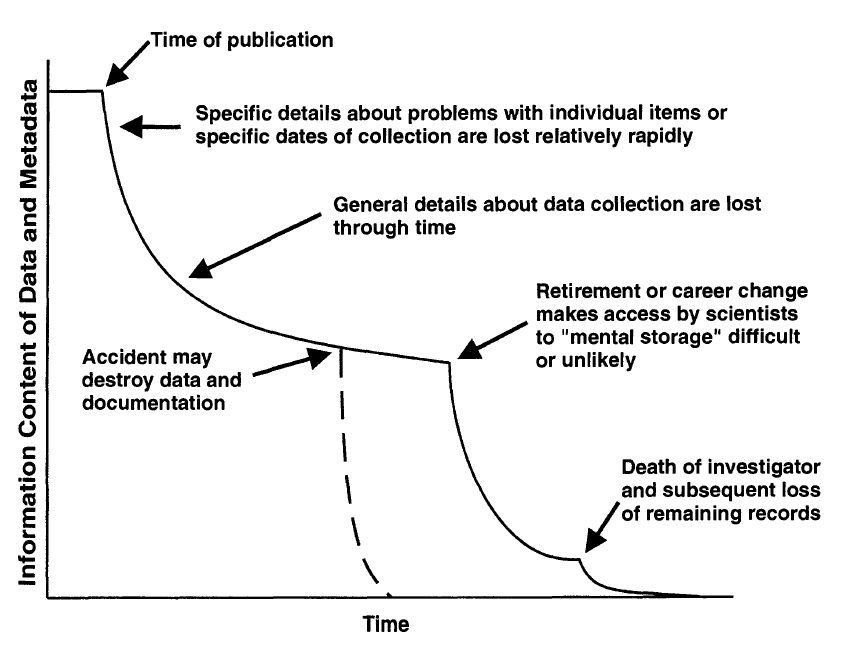
\includegraphics{death.png}
\caption{Bill Michener's description of data completeness over time}
\end{figure}

\section{Data processing \& analysis}\label{data-processing-analysis}

\subsection{What does this stage
involve?}\label{what-does-this-stage-involve-2}

These stages are in separate boxes on the lifecycle model, and they may
indeed be different steps, but not always. You usually process data in
order to get to an analyzable form of it. The stages have the same
considerations. This stage includes any data cleaning, refinement,
integration, and organizing (combining variables, weighting variables)
that you might do, as well as any computation necessary for analysis.

\subsection{What tools and resources are
available?}\label{what-tools-and-resources-are-available-2}

\paragraph{\href{http://csssi.yale.edu/tech}{Software}:}\label{software}

\begin{itemize}
\itemsep1pt\parskip0pt\parsep0pt
\item
  Stata
\item
  SAS
\item
  MatLab
\item
  R
\item
  OpenRefine
\item
  Python
\item
  \href{http://www.dataone.org/software_tools_catalog}{DataONE software
  tools catalog}
\end{itemize}

\paragraph{\href{http://statlab.stat.yale.edu/workshops/}{CSSSI
Workshops}}\label{csssi-workshops}

\paragraph{\href{http://its.yale.edu/services/research-technologies/high-performance-computing}{High
Performance Computing}}\label{high-performance-computing}

\paragraph{\href{http://guides.library.yale.edu/gis}{Geographic
Information Systems}}\label{geographic-information-systems}

\paragraph{Workflow tools}\label{workflow-tools}

\begin{itemize}
\itemsep1pt\parskip0pt\parsep0pt
\item
  \href{https://kepler-project.org/}{Kepler}:
  https://kepler-project.org/ : open source scientific workflow
  application.
\item
  \href{http://www.vistrails.org/index.php/Main_Page}{VisTrails}:
  http://www.vistrails.org : open source scientific workflow
  application, emphasis on visualization.
\end{itemize}

\subsection{People:}\label{people}

\paragraph{Steve Weston, HPC
specialist}\label{steve-weston-hpc-specialist}

Steve has office hours in the CSSSI from 9:30 - 1:00 on Wednesdays.

\paragraph{Stace Maples, GIS
specialist}\label{stace-maples-gis-specialist}

Stace has office hours in the CSSSI, the med library, and HGS. Find out
more here: \url{http://guides.library.yale.edu/gis}

\paragraph{StatLab consultants:}\label{statlab-consultants-1}

StatLab consultants staff a desk in the CSSSI. Their schedules are:
\url{http://csssi.yale.edu/csssi-statistical-consultants-schedule}

\paragraph{Kristin Bogdan \& Michelle Hudson, Data
Librarians}\label{kristin-bogdan-michelle-hudson-data-librarians}

Kristin \& Michelle have offices in CSSSI, and you can see their offsite
office hours at: \url{http://bit.ly/datalibofficehours}

\subsection{Guidelines:}\label{guidelines-1}

\begin{enumerate}
\def\labelenumi{\arabic{enumi}.}
\itemsep1pt\parskip0pt\parsep0pt
\item
  Keep track of everything you do and always keep versions of your data
  sets.
\item
  Best practices for working with data during analysis -- folder
  structures, naming conventions, statistical package considerations.
\item
  How to back up data.
\end{enumerate}

\section{Data archiving \&
preservation}\label{data-archiving-preservation}

\subsection{What does this stage
involve?}\label{what-does-this-stage-involve-3}

Archiving and preserving research data is different from distributing it
or backing it up regularly. Preservation ensures long-term retention of
the data and the necessary migration from format to format that will be
required to keep the data usable over a time period. How long you retain
your data is often up to what your funding dictates -- some grants say
three years, others five. In some cases, your data may have value for an
indefinite period of time.

\subsection{What tools and resources are
available?}\label{what-tools-and-resources-are-available-3}

\paragraph{Lists of repositories:}\label{lists-of-repositories}

A few projects aim to list all the data repositories available for
submission or for finding research data to reuse, and you can search or
browse by subject:  

\begin{itemize}
\itemsep1pt\parskip0pt\parsep0pt
\item
\href{http://databib.org/}{DataBib} 
\item
\href{http://www.re3data.org}{re3data}
\end{itemize}

\subsection{Guidelines:}\label{guidelines-2}

\begin{enumerate}
\def\labelenumi{\arabic{enumi}.}
\itemsep1pt\parskip0pt\parsep0pt
\item
  Doing preservation yourself requires format migration and ensuring
  integrity of files.
\item
  Handing over your data to a repository like ICPSR is possible, and
  will ensure the data is usable over the long-term.
\end{enumerate}

\subsection{Examples:}\label{examples}

\paragraph{\href{http://isps.yale.edu/research\#.UwJU7IVnCSo}{Institution
for Social \& Policy
Studies}}\label{institution-for-social-policy-studies}

ISPS is a Yale department that maintains a data archive of research that
has been conducted by their affiliates.

\paragraph{\href{http://icpsr.umich.edu}{ICPSR}}\label{icpsr}

The Inter-university Consortium for Political and Social research is a
domain archive that has been curating and maintaining access to data
sets for over 50 years.

\section{Data distribution \&
citation}\label{data-distribution-citation}

\subsection{What does this stage
involve?}\label{what-does-this-stage-involve-4}

This is the stage (usually after archiving) where you can make your
data, or a link to your data available, so that others know they can get
your raw materials and use them in their own research, or check your
studies for replication.

\subsection{What tools and resources are
available?}\label{what-tools-and-resources-are-available-4}

\paragraph{\href{https://www.datacite.org/}{DataCite}}\label{datacite}

\paragraph{Repositories (listed above)}\label{repositories-listed-above}

\subsection{Guidelines:}\label{guidelines-3}

\begin{enumerate}
\def\labelenumi{\arabic{enumi}.}
\itemsep1pt\parskip0pt\parsep0pt
\item
  Give your data set a title and make it easy to credit you.
\item
  Always cite data that you use as if it were as important as the
  journal articles you cite.
\end{enumerate}

\subsection{Examples:}\label{examples-1}

\begin{enumerate}
\def\labelenumi{\arabic{enumi}.}
\itemsep1pt\parskip0pt\parsep0pt
\item
  ICPSR data citation
\item
  DataCite data citation
\end{enumerate}

\section{References \& other
resources:}\label{references-other-resources}

\paragraph{\href{http://library.umassmed.edu/necdmc/index}{NECDMC}}\label{necdmc}

Some material from this presentation came from the New England
Collaborative Data Management Curriculum.

\paragraph{\href{http://datalib.edina.ac.uk/mantra/}{MANTRA}}\label{mantra}

Mantra is series of useful research data management training modules you
can complete online.

\paragraph{Guides \& links}\label{guides-links}

These guides may be useful as you work on your projects: 

\begin{itemize}
\itemsep1pt\parskip0pt\parsep0pt
\item
\url{http://guides.library.yale.edu/datamanagement} 
\item
\url{http://guides.library.yale.edu/data-statistics} 
\item
\url{http://guides.library.yale.edu/sciencedata} 
\item
\url{http://guides.library.yale.edu/eln} 
\item
\url{http://csssi.yale.edu/datamanagement}
\end{itemize}

\section{Contact info}\label{contact-info}

\subsubsection{Michelle Hudson}\label{michelle-hudson}

\begin{itemize}
\itemsep1pt\parskip0pt\parsep0pt
\item
  Science and Social Science Data Librarian
\item
  203.432.4587
\item
  \url{michelle.hudson@yale.edu}
\item
  office hours: \url{http://bit.ly/datalibofficehours}
\end{itemize}

\subsubsection{Kristin Bogdan}\label{kristin-bogdan}

\begin{itemize}
\itemsep1pt\parskip0pt\parsep0pt
\item
  Science and Social Science Data Librarian
\item
  203.436.5907
\item
  \url{kristin.bogdan@yale.edu}
\item
  office hours: \url{http://bit.ly/datalibofficehours}
\end{itemize}

\subsubsection{StatLab Consultants}\label{statlab-consultants-2}

\begin{itemize}
\itemsep1pt\parskip0pt\parsep0pt
\item
  Schedule:
  \url{http://csssi.yale.edu/csssi-statistical-consultants-schedule}
\item
  203.432.3277
\end{itemize}

\end{document}
